\documentclass[acmsmall,screen]{acmart}
\usepackage{booktabs}
\settopmatter{printacmref=false}
\renewcommand\footnotetextcopyrightpermission[1]{}
\setcopyright{none}
\acmConference{}{}{}
\acmJournal{CSUR}\acmYear{2026}\acmVolume{1}\acmNumber{1}\acmArticle{1}\acmMonth{10}
\citestyle{acmauthoryear}

\begin{document}
\title{Negative-Flip-Aware Model Updates under Controlled Drift: A Comparative Study of Weight Interpolation and a Consistency-Penalty Baseline}
\author{Narayan Gurjar}
\affiliation{\institution{Roll No.\ MSE2026002 --- AI Tools for Research, Lab 02}\city{Kanpur}\country{India}}
\renewcommand{\shortauthors}{Gurjar}

\begin{abstract}
My earlier literature review on performance drift across large-language-model updates identified the \emph{negative flip}---an input handled correctly before an update and incorrectly after---as the common unit of update regression, and two families of mitigation (training-time consistency penalties and post-hoc weight interpolation) that are each evaluated only against their own baselines. No commercial LLM API or GPU was available, so I move one level down the review's taxonomy to a fully reproducible testbed: a from-scratch softmax classifier on the scikit-learn digits data, where the ``update'' is retraining on training images corrupted by Gaussian noise of strength $\sigma$. Under one frozen protocol (validation-based hyperparameter selection, a fixed held-out test set, 5 seeds), I compare naive retraining, a simplified PCT-style consistency penalty, and backward-compatible weight interpolation (BCWI). Weight interpolation reduced test negative flip rate relative to naive retraining at every $\sigma$ and in all 5 seeds (e.g.\ $0.085\to0.046$ at $\sigma{=}8$), but its benefit is largely a shrinkage toward the old model and, for $\sigma\ge 6$, accuracy still falls below that of simply keeping the old model. The simplified consistency penalty did \emph{not} help: it never reduced flips reliably (equal at small $\sigma$, higher at large $\sigma$). These results come from a single small linear testbed and say nothing directly about LLMs.
\end{abstract}
\keywords{negative flips, backward compatibility, model updates, weight interpolation, drift}
\maketitle

\section{Introduction}
Deployed models are updated, and an update that raises aggregate accuracy can still break inputs that previously worked. Chen et al.~\cite{chen2024chatgpt} documented large behavior changes between two snapshots of commercial LLM services, and Echterhoff et al.~\cite{echterhoff2024muscle} measured instance-level regression when an LLM's base model is updated. Both lean on the \emph{negative flip} notion introduced for human--AI teams by Bansal et al.~\cite{bansal2019updates}.

\paragraph{Link to my literature review.} My review (Paper~1) argued that (i) the negative flip rate (Eq.~\ref{eq:nfr}) is the natural unit of update regression, (ii) positive-congruent training~\cite{yan2021positive} and weight interpolation~\cite{schumann2024backward} are the main mitigations, and (iii) drift studies use heterogeneous, study-specific metrics. A direct reproduction of the LLM audits is not possible here: the audited snapshots are not available to me and the sandbox has neither model-API access nor a GPU. I therefore study the mitigation question in a controlled classical setting. The contribution is a \emph{routine comparison under a shared protocol}; I make no claim of algorithmic novelty.

\section{Background}
\textbf{Concept drift} is a change in the joint distribution $P(X,Y)$ over time~\cite{gama2014survey}. In model updates the roles reverse: inputs are stable while the \emph{model} changes. Given old and new classifiers $f_o,f_n$ and a labelled set $D$,
\begin{equation}
\mathrm{NFR}(f_o,f_n,D)=\frac{|\{x\in D: f_o(x)=y\,\wedge\,f_n(x)\neq y\}|}{|D|},
\label{eq:nfr}
\end{equation}
and the positive flip rate (PFR) swaps the two conditions. Regression bugs in NLP model updates were measured by Xie et al.~\cite{xie2021regression}. \citet{yan2021positive} propose positive-congruent training, which penalizes new-model errors on inputs the old model got right. \citet{schumann2024backward} propose backward-compatible weight interpolation (BCWI). Catastrophic forgetting~\cite{kirkpatrick2017overcoming} is the related continual-learning view.

\section{Research Questions and Success Criterion}
\textbf{RQ.} In a controlled testbed, how do a PCT-style consistency penalty and BCWI compare with naive retraining in the accuracy--NFR trade-off, and how does this change with the magnitude of the update?
\begin{itemize}
\item \textbf{SQ1} Which method gives lower NFR at a strong update ($\sigma{=}8$)?
\item \textbf{SQ2} How does the advantage change with $\sigma$?
\item \textbf{SQ3} Which classes carry the residual flips?
\end{itemize}
\textbf{Hypotheses (before the sweep):} H1: BCWI reduces NFR relative to NAIVE. H2: the PCT-style penalty reduces NFR. \textbf{Criterion (written before the final sweep, after exploratory pilots):} a setting is ``useful'' if mean validation NFR falls $\ge 20\%$ versus NAIVE at $\le 2$ points of accuracy cost.

\section{Method}
\paragraph{Testbed.} A multinomial logistic regression written in NumPy (SGD, 300 epochs, lr 0.5, batch 64, L2 $10^{-4}$) on \texttt{sklearn.datasets.load\_digits} (1797 images, 64 features, 10 classes; offline, BSD-licensed package). Old and new models share the same initial weights (needed for interpolation).
\paragraph{Update proxy.} The old model $f_o$ is trained on a clean 25\% subsample of the training pool. The new model sees 100\% of the pool, with additive Gaussian noise (std $\sigma$, pixels clipped to $[0,16]$) applied to every training image; $\sigma{=}0$ is a clean data-growth update. Evaluation images are never corrupted. This is an \emph{inferred proxy} for a real update, not an LLM update.
\paragraph{Comparators.}
\textbf{NAIVE}: retrain with cross-entropy. \textbf{PCT-style}: add to the loss a penalty pushing the new model's output toward the old model's prediction on training rows the old model classified correctly,
\begin{equation}
\mathcal{L}=\mathrm{CE}(y,p_\theta)+\lambda\,\mathbb{1}[f_o(x)=y]\,\mathrm{CE}(f_o(x),p_\theta).
\label{eq:pct}
\end{equation}
This is a simplified variant written by me, \emph{not} a verified reproduction of \citet{yan2021positive}. \textbf{BCWI}: train NAIVE, then interpolate parameters,
\begin{equation}
\theta_{\alpha}=\alpha\,\theta_o+(1-\alpha)\,\theta_n,
\label{eq:bcwi}
\end{equation}
so $\alpha{=}0$ is NAIVE and $\alpha{=}1$ is the old model. A frozen OLD model is reported as a reference.
\paragraph{Protocol.} Per seed, a stratified 20\% test set is fixed and never used for selection; 20\% of the remainder is a validation set. $\lambda\in\{0,.25,.5,1,2,4\}$ and $\alpha\in\{0,.2,\dots,.95,.98,1\}$ are chosen \emph{once}, on validation at $\sigma{=}8$, then held fixed for all $\sigma\in\{0,2,\dots,10\}$. $\alpha{=}1$ is excluded from selection (it is the old model, not an update). Seeds $0$--$4$; all numbers are mean$\pm$std over seeds.

\section{Experiments}
\subsection{Baseline validation}
Before any comparison, I checked that the dataset loads offline, that test and training indices are disjoint, that training loss falls, and that NFR is non-trivial (reference seed 42: OLD 0.928 and NAIVE 0.961 accuracy, 3 of 360 test images flipped negatively; logs in \texttt{results/logs}). These are sanity checks of my own implementation, not a reproduction of published numbers; no published result for this testbed exists to compare against.

\subsection{Ablation (validation split, $\sigma{=}8$)}
Table~\ref{tab:abl} and Fig.~\ref{fig:tradeoff} show the sweeps. Every PCT-style setting had higher NFR \emph{and} lower accuracy than NAIVE; no $\lambda$ met the criterion. BCWI met it for $\alpha\ge0.95$; the rule selected $\alpha^*{=}0.98$, which lies at the edge of the grid next to the degenerate $\alpha{=}1$.
\begin{table}[t]\centering\small
\caption{Validation-split ablation at $\sigma{=}8$ (mean over 5 seeds). NFR change is relative to NAIVE (val.\ NFR 0.082, accuracy 0.874; frozen OLD accuracy 0.931).}\label{tab:abl}
\begin{tabular}{llccc}
\toprule
Method & Setting & Val.\ acc. & Val.\ NFR & NFR change vs.\ NAIVE \\
\midrule
PCT & $\lambda{=}0.25$ & 0.857 & 0.101 & +22.9\% \\
PCT & $\lambda{=}1$ & 0.795 & 0.162 & +98.3\% \\
PCT & $\lambda{=}4$ & 0.702 & 0.255 & +211.0\% \\
BCWI & $\alpha{=}0.8$ & 0.877 & 0.078 & -5.1\% \\
BCWI & $\alpha{=}0.9$ & 0.887 & 0.068 & -16.9\% \\
BCWI & $\alpha{=}0.95$ & 0.895 & 0.060 & -26.3\% \\
BCWI & $\alpha{=}0.98$ & 0.913 & 0.040 & -50.8\% \\
\bottomrule
\end{tabular}
\end{table}
\begin{figure}[t]\centering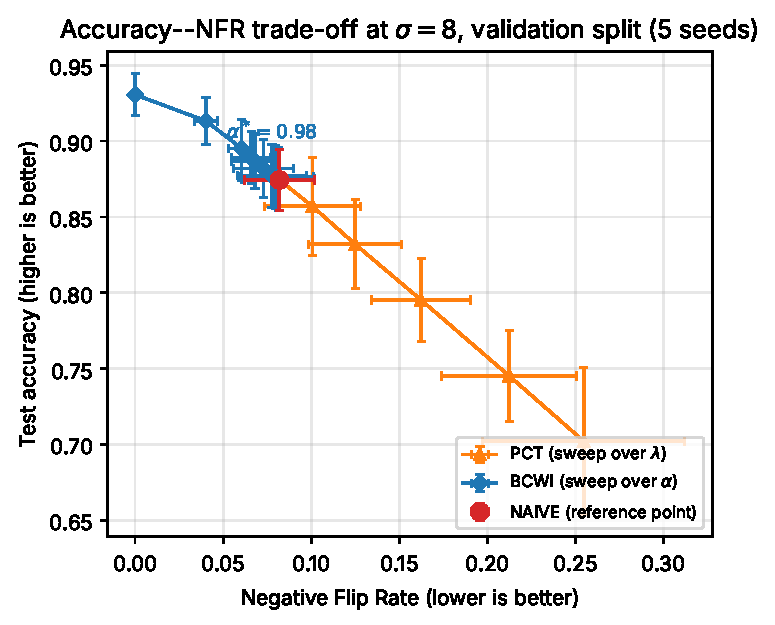
\includegraphics[width=.6\linewidth]{figures/fig1_tradeoff_ablation.pdf}
\caption{Validation accuracy--NFR trade-off at $\sigma{=}8$ over PCT $\lambda$ and BCWI $\alpha$ (error bars: std over seeds).}\label{fig:tradeoff}\end{figure}

\subsection{Magnitude sweep (test split)}
Tables~\ref{tab:nfr} and~\ref{tab:acc} and Figs.~\ref{fig:nfr}--\ref{fig:acc} give test results with $\lambda{=}0.25$ (mildest tested value, carried to check the negative result across $\sigma$) and $\alpha^*{=}0.98$.
\begin{table}[t]\centering\small
\caption{Test negative flip rate (lower is better).}\label{tab:nfr}\begin{tabular}{lcccc}
\toprule
$\sigma$ & OLD (frozen) & NAIVE & PCT ($\lambda{=}0.25$) & BCWI ($\alpha^*$) \\
\midrule
0 & 0.000$\pm$0.000 & 0.014$\pm$0.010 & 0.014$\pm$0.010 & 0.000$\pm$0.000 \\
2 & 0.000$\pm$0.000 & 0.019$\pm$0.008 & 0.019$\pm$0.007 & 0.004$\pm$0.002 \\
4 & 0.000$\pm$0.000 & 0.037$\pm$0.008 & 0.038$\pm$0.013 & 0.016$\pm$0.001 \\
6 & 0.000$\pm$0.000 & 0.059$\pm$0.006 & 0.067$\pm$0.008 & 0.029$\pm$0.003 \\
8 & 0.000$\pm$0.000 & 0.085$\pm$0.010 & 0.094$\pm$0.014 & 0.046$\pm$0.004 \\
10 & 0.000$\pm$0.000 & 0.097$\pm$0.012 & 0.118$\pm$0.019 & 0.052$\pm$0.007 \\
\bottomrule
\end{tabular}\end{table}
\begin{table}[t]\centering\small
\caption{Test accuracy (higher is better).}\label{tab:acc}\begin{tabular}{lcccc}
\toprule
$\sigma$ & OLD (frozen) & NAIVE & PCT ($\lambda{=}0.25$) & BCWI ($\alpha^*$) \\
\midrule
0 & 0.935$\pm$0.010 & 0.965$\pm$0.012 & 0.964$\pm$0.012 & 0.937$\pm$0.011 \\
2 & 0.935$\pm$0.010 & 0.951$\pm$0.011 & 0.952$\pm$0.010 & 0.944$\pm$0.010 \\
4 & 0.935$\pm$0.010 & 0.923$\pm$0.012 & 0.921$\pm$0.018 & 0.941$\pm$0.009 \\
6 & 0.935$\pm$0.010 & 0.896$\pm$0.011 & 0.886$\pm$0.015 & 0.926$\pm$0.011 \\
8 & 0.935$\pm$0.010 & 0.869$\pm$0.008 & 0.859$\pm$0.013 & 0.907$\pm$0.013 \\
10 & 0.935$\pm$0.010 & 0.856$\pm$0.009 & 0.834$\pm$0.013 & 0.901$\pm$0.012 \\
\bottomrule
\end{tabular}\end{table}
\begin{table}[t]\centering\small
\caption{Seeds (of 5) in which a method's test NFR is strictly below NAIVE's. No significance test is claimed.}\label{tab:seed}\begin{tabular}{lcc}
\toprule
$\sigma$ & BCWI $<$ NAIVE (seeds) & PCT $<$ NAIVE (seeds) \\
\midrule
0 & 5/5 & 1/5 \\
2 & 5/5 & 2/5 \\
4 & 5/5 & 3/5 \\
6 & 5/5 & 0/5 \\
8 & 5/5 & 1/5 \\
10 & 5/5 & 0/5 \\
\bottomrule
\end{tabular}\end{table}
\begin{figure}[t]\centering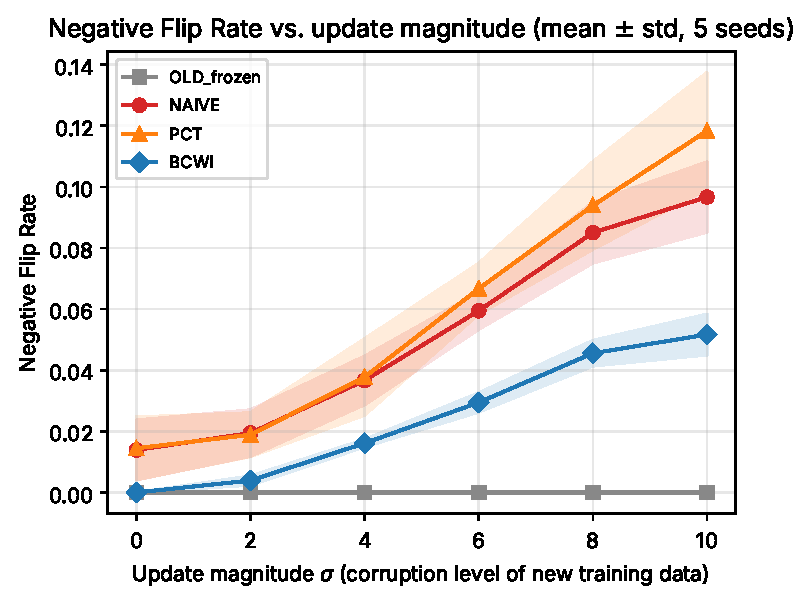
\includegraphics[width=.6\linewidth]{figures/fig2_nfr_vs_sigma.pdf}\caption{Test NFR versus update magnitude $\sigma$ (band: $\pm$1 std).}\label{fig:nfr}\end{figure}
\begin{figure}[t]\centering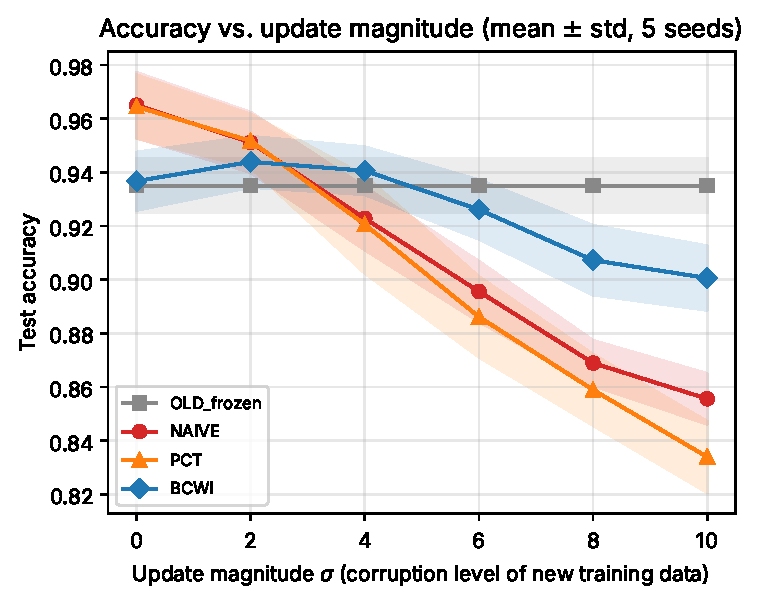
\includegraphics[width=.6\linewidth]{figures/fig3_accuracy_vs_sigma.pdf}\caption{Test accuracy versus $\sigma$. NAIVE and PCT fall below the frozen OLD model as $\sigma$ grows.}\label{fig:acc}\end{figure}

\subsection{Failure analysis ($\sigma{=}8$, test)}
Summed over 5 seeds (1800 test evaluations), NAIVE produced 153 negative flips and BCWI 82 (a 46\% reduction). Both concentrate on the same classes (Fig.~\ref{fig:class}): digit 8 (56 $\to$ 29), digit 9 (29 $\to$ 17) and digit 1 (21 $\to$ 14), i.e.\ interpolation shrinks, but does not relocate, the regressions.
\begin{figure}[t]\centering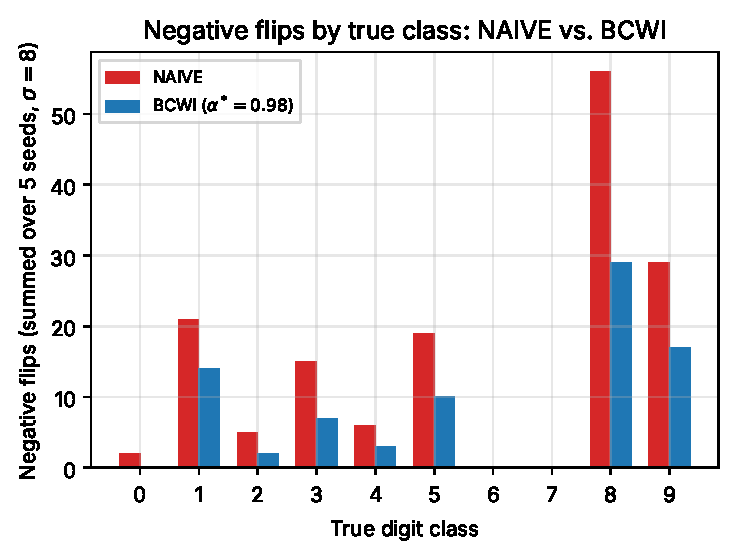
\includegraphics[width=.6\linewidth]{figures/fig4_failure_by_class.pdf}\caption{Negative flips by true class at $\sigma{=}8$, summed over seeds.}\label{fig:class}\end{figure}

\section{Discussion}
\textbf{SQ1/H1.} BCWI had lower test NFR than NAIVE at every $\sigma$ in all 5 seeds (Table~\ref{tab:seed}); at $\sigma{=}8$, $0.046$ versus $0.085$. H1 is supported in this testbed. \textbf{H2 is contradicted:} the PCT-style penalty was never reliably below NAIVE (at most 3/5 seeds, and 0/5 at $\sigma{=}6,10$) and its NFR and accuracy worsened as $\sigma$ grew. A plausible but untested explanation is that a hard-label penalty on old-correct rows conflicts with fitting the corrupted new data and adds no information beyond the cross-entropy term; I did not run an experiment to confirm this, and my variant may simply be a poor implementation of the published idea.

\textbf{SQ2 and an important caveat.} The BCWI advantage in NFR grows with $\sigma$ in absolute terms, but it must be read against the frozen OLD model. At $\sigma{=}0$ BCWI's accuracy (0.937) is essentially that of OLD (0.935) with zero flips: with $\alpha^*{=}0.98$ the merged model is almost the old model, so a low NFR is expected. A useful update should also improve accuracy; BCWI exceeds OLD only marginally at $\sigma\le 4$, and at $\sigma\le 2$ NAIVE is clearly more accurate than BCWI (0.965 vs.\ 0.937 at $\sigma{=}0$), so BCWI pays an accuracy price when the update is benign; and for $\sigma\ge6$ its accuracy is below OLD's (e.g.\ 0.907 vs.\ 0.935 at $\sigma{=}8$). In that regime keeping the old model beats all three updates. The result therefore does not show BCWI ``solves'' update regression; it shows it trades a small share of the update's gain for much fewer flips, whereas PCT-style training here only paid costs.

\section{Limitations}
(1) One dataset, one linear model, synthetic noise as the drift proxy; no claim about LLMs, RLHF, instruction following or sycophancy. (2) PCT is a simplified, unverified variant. (3) $\alpha^*$ sits at the grid edge; a finer grid between 0.98 and 1 was not tried. (4) Five seeds and no formal significance testing. (5) Trainer hyperparameters were fixed, not tuned. (6) The success criterion was fixed after exploratory pilots, so it is not a pre-registered threshold. (7) The code is AI-assisted and only sanity-tested (see \texttt{ai\_assistance\_log.md}).

\section{Conclusion}
Under one frozen protocol, weight interpolation lowered negative flips relative to naive retraining while a simplified consistency penalty did not, but interpolation's gains largely reflect staying near the old model. Natural follow-ups, ranked by cost: a faithful PCT implementation checked against the original; a finer $\alpha$ grid with a requirement of beating OLD accuracy; and a small open-weight LLM update study.

\paragraph{Reproducibility.} Code, configs, seeds, logs and commands are in the accompanying repository (\texttt{README.md}); the full pipeline runs on CPU in minutes.

\bibliographystyle{ACM-Reference-Format}
\bibliography{references}
\end{document}
